\section{HiFi-forstærkerens generelle opbygning}

En HiFi-forstærker kan være opbygget på forskellige måder, som blandt andet er afhængig af kravene til indgangstyper, harmonisk forvrængning og strømforbrug. Derudover kan forskellige designs afvige fra hinanden alt efter hvilke funktioner der inkluderes, såsom; volumenkontrol, equalizer

Forskellige byggeblokke

Hvad skal der tages hensyn til når man designer en HiFi-forstærker?



\begin{figure}[h]
\centering
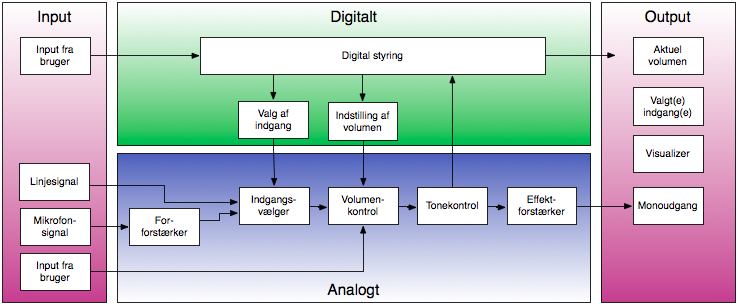
\includegraphics[scale=.6]{indledende_analyse/generel_effektforstaerker/forstaerker_opbygning.png}
\caption{Opbygning af HiFi-forstærker}
\label{}
\end{figure}